% !TEX encoding = UTF-8
% !TEX TS-program = pdflatex
% !TEX root = ../tesi.tex

%**************************************************************
\chapter{Analisi dei requisiti}
\label{cap:analisi-requisiti}
%**************************************************************

\intro{Breve introduzione al capitolo}\\

\section{Casi d'uso}

Per lo studio dei casi di utilizzo del prodotto sono stati creati dei diagrammi.
I diagrammi dei casi d'uso (in inglese \emph{Use Case Diagram}) sono diagrammi di tipo \gls{uml} dedicati alla descrizione delle funzioni o servizi offerti da un sistema, così come sono percepiti e utilizzati dagli attori che interagiscono col sistema stesso.
Essendo il progetto finalizzato alla creazione di un tool per l'automazione di un processo di decompilazione di un file APK, di trasformazione dei file decompilati (\textit{dex}) in codice java e dell'analisi di quest'ultimo.



\subsection{Attori}\label{sec:attori}
L'unico utilizzatore del software \`{e} identificato come \textbf{attore generico}, ha il permesso di effettuare tutte le operazioni offerte dal tool.

\subsection{Casi d'uso}\label{subsec:casi-d'uso}
\subsubsection{UC-1 Selezione file}\label{subsubsec:uc-1-selezione-file}
\begin{itemize}
    \item \textbf{attori:} utente generico;
    \item \textbf{scopo:} permettere all'utente di selezionare il file APK da analizzare;
    \item \textbf{descrizione:} serve per permettere all'utente di selezionare il file APK da analizzare;
    \item \textbf{pre-condizioni:} l'utente ha avviato il tool;
    \item \textbf{post-condizioni:} l'utente ha selezionato un file di con estensione \textbf{.APK} valido;
    \item \textbf{flusso degli eventi principali:}
    \begin{itemize}
        \item l'utente seleziona il file;
        \item l'utente conferma la selezione del file.
    \end{itemize}
\end{itemize}
\subsubsection{UC-2 Avvio decompilazione}\label{subsubsec:uc-2-avvio-decompilazione}
\begin{itemize}
    \item \textbf{attori:} utente generico;
    \item \textbf{scopo:} serve per avviare la decompilazione;
    \item \textbf{descrizione:} l'utente deve avviare la decompilazione del file APK;
    \item \textbf{pre-condizioni:} l'utente ha selezionato con successo un file APK;
    \item \textbf{post-condizioni:} la decompilazione è avvenuto con successo;
    \item \textbf{flusso degli eventi principali:}
    \begin{itemize}
        \item l'utente avvia la decompilazione;
        \item l'utente visualizza il messaggio della decompilazione avvenuto con successo;
    \end{itemize}
    \item \textbf{Estensione:}
    \begin{itemize}
        \item UC-3 Visualizzazione errore di decompilazione;
    \end{itemize}
\end{itemize}

\subsubsection{UC-3 Visualizzazione errore di decompilazione}\label{subsubsec:uc-3-visualizzazione-errore-di-decompilazione}
\begin{itemize}
    \item \textbf{attori:} utente generico;
    \item \textbf{scopo:} mostrare il messaggio d'errore della decompilazione;
    \item \textbf{descrizione:} la decompilazione del file APK potrebbe generare degli errori;
    \item \textbf{pre-condizioni:} l'utente ha avviato la decompilazione dell'APK;
    \item \textbf{post-condizioni:} l'utente ha visualizzato il messaggio d'errore;
    \item \textbf{flusso degli eventi principali:}
    \begin{itemize}
        \item l'utente visualizza il messaggio di errore;
    \end{itemize}
\end{itemize}
\subsubsection{UC- 4 Installazione APK decompilato}\label{subsubsec:uc--4-installazione-APK-decompilato}
\begin{itemize}
    \item \textbf{attori:} utente generico;
    \item \textbf{scopo:} installazione dell'APK decompilato su un AVD;
    \item \textbf{descrizione:} permette all'utente d'installare l'apk, decompilato, manomesso e ricompilato, su un AVD;
    \item \textbf{pre-condizioni:} la decompilazione dell'APK è stato eseguito con successo;
    \item \textbf{post-condizioni:} l'APK è stato installato sull'AVD con successo;
    \item \textbf{flusso degli eventi principali:}
    \begin{itemize}
        \item l'utente seleziona un'AVD presente sul proprio computer;
        \item l'utente avvia l'installazione dell'APK ricompilato;
        \item l'utente visualizza un messaggio d'installazione avvenuto con successo;
    \end{itemize}
\end{itemize}
\subsubsection{UC- 4.1 Selezione AVD}\label{subsubsec:uc--4.1-selezione-avd}
\begin{itemize}
    \item \textbf{attori:} utente generico;
    \item \textbf{scopo:} permettere all'utente di selezionare i AVD presenti nel proprio computer;
    \item \textbf{descrizione:} serve per permettere all'utente di selezionare un'AVD presente nel proprio computer;
    \item \textbf{pre-condizioni:} l'utente ha avviato il software;
    \item \textbf{post-condizioni:} l'utente ha selezionato l'AVD da avviare;
    \item \textbf{flusso degli eventi principali:}
    \begin{itemize}
        \item l'utente visualizza un elenco delle AVD presenti nel proprio computer;
        \item l'utente seleziona un'AVD;
        \item l'utente conferma la selezione;
        \item l'AVD selezionato si è avviato con successo
    \end{itemize}
    \item \textbf{Estensione}
    \begin{itemize}
        \item UC-5 Visualizzazione messaggio nessun AVD rilevato;
    \end{itemize}
\end{itemize}
\begin{figure}
    \centering
    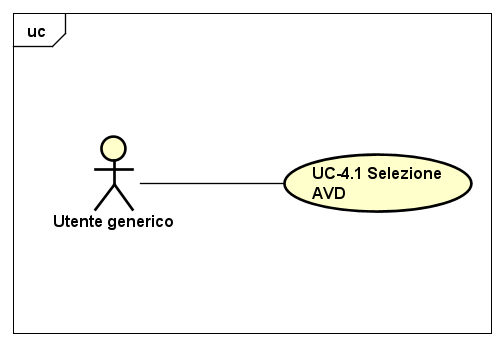
\includegraphics[width=10cm, height=8cm]{./usecase/uc_4_1.png}
    \caption{UC-4.1 Selezione AVD}
\end{figure}

\subsubsection{UC-5 Visualizzazione messaggio nessun AVD rilevato} \label{subsubsec:uc-5-visualizzazione-messaggio-nessun-avd-rilevato}
\begin{itemize}
    \item \textbf{attori:} utente generico;
    \item \textbf{scopo:} mostrare all'utente che non sono stati rilevati alcun AVD;
    \item \textbf{descrizione:} quando non sono presenti nessun AVD o il tool non è riuscito a rilevarne, viene mostrato un messaggio all'utente;
    \item \textbf{pre-condizioni:} l'utente ha aperto il tool;
    \item \textbf{post-condizioni:} l'utente ha visualizzato il messaggio;
    \item \textbf{flusso degli eventi principali:}
    \begin{itemize}
        \item l'utente visualizza il messaggio;
    \end{itemize}
\end{itemize}
\subsubsection{UC-6 Errore durante avvio dell'AVD}\label{subsubsec:uc-6-errore-durante-avvio-dell'avd}
\begin{itemize}
    \item \textbf{attori:} utente generico;
    \item \textbf{scopo:} mostrare all'utente gli eventuali errori durante l'avvio dell'AVD;
    \item \textbf{descrizione:} serve a mostrare all'utente gli eventuali errori durante l'avvio dell'AVD;
    \item \textbf{pre-condizioni:} l'utente ha selezionato un'AVD e ha confermato l'avvio;
    \item \textbf{post-condizioni:} l'utente ha visualizzato il messaggio d'errore;
    \item \textbf{flusso degli eventi principali:}
    \begin{itemize}
        \item l'utente visualizza il messaggio d'errore;
    \end{itemize}
\end{itemize}
\subsubsection{UC-7 Dump dello storage interno}\label{subsubsec:uc-6-dump-dello-storage-interno}
\begin{itemize}
    \item \textbf{attori:} utente generico;
    \item \textbf{scopo:} permettere all'utente di fare il dump dello storage interno;
    \item \textbf{descrizione:} nel caso l'utente volesse una copia dei dati interni dell'applicativo, ha bisogno di fare il dump;
    \item \textbf{pre-condizioni:} l'installazione dell'APK manomesso è andato a buon fine;
    \item \textbf{post-condizioni:} è stato fatto una copia dello storage interno;
    \item \textbf{flusso degli eventi principali:}
    \begin{itemize}
        \item l'utente seleziona la voce "copia i dati interni";
        \item l'utente seleziona il path dove collocare i dati;
    \end{itemize}
\end{itemize}
\subsubsection{UC-8 Decodifica del codice}\label{subsubsec:uc-8-decodifica-del-codice}
\begin{itemize}
    \item \textbf{attori:} utente generico;
    \item \textbf{scopo:} permettere all'utente di effettuare la decodifica dei file \textbf{.dex} in codice \textbf{.java};
    \item \textbf{descrizione:} durante la decompilazione dell'APK vengono creati dei file .dex che contengono il codice sorgente dell'APK, e questo caso d'uso serve per permettere all'utente di ottenere il codice sorgente;
    \item \textbf{pre-condizioni:} la decompilazione è avvenuto con successo;
    \item \textbf{post-condizioni:} l'utente ha ottenuto una copia del codice sorgente in java;
    \item \textbf{flusso degli eventi principali:}
    \begin{itemize}
        \item l'utente ha selezionato la funzionalità decodifica dei dex;
        \item l'utente seleziona il percorso dove posizionare il codice sorgente ottenuto;
        \item l'utente ha salvato il codice sorgente ottenuto.
    \end{itemize}
\end{itemize}
\subsubsection{UC-8.1 Avvio decodifica}
\begin{itemize}
    \item \textbf{attori:} utente generico;
    \item \textbf{scopo:} serve all'utente per avviare la decodifica dei file .dex;
    \item \textbf{descrizione:} serve all'utente per avviare la decodifica dei file .dex;
    \item \textbf{pre-condizioni:} la decompilazione dell'APK è avvenuto correttamente;
    \item \textbf{post-condizioni:} la decodifica è avvenuto con successo;
    \item \textbf{flusso degli eventi principali:}
    \begin{itemize}
        \item l'utente seleziona la funzionalità di decodifica dei file .dex;
    \end{itemize}
\end{itemize}
\subsubsection{UC-8.2 Salvataggio del codice decodificato}
\begin{itemize}
    \item \textbf{attori:} utente generico;
    \item \textbf{scopo:} serve all'utente per salvare i codici sorgenti decodificati;
    \item \textbf{descrizione:} serve all'utente per salvare i codici sorgenti decodificati;
    \item \textbf{pre-condizioni:} la decompilazione è avvenuto con successo;
    \item \textbf{post-condizioni:} i file con i codici sorgenti sono stati salvati correttamente;
    \item \textbf{flusso degli eventi principali:}
    \begin{itemize}
        \item l'utente seleziona la voce "salva file decodificati";
        \item l'utente seleziona la posizione dove vuole salvare i file;
        \item i file vengono salvati correttamente.
    \end{itemize}
\end{itemize}

\begin{figure}[H]
    \centering
    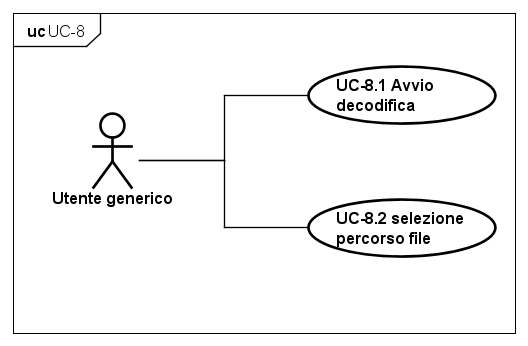
\includegraphics[width=10cm, height=8cm]{./immagini/usecase/uc_8.png}
    \caption{UC-8 Decodifica codici .dex}
\end{figure}



\subsubsection{UC-9 Visualizzazione errore decodifica}\label{subsubsec:uc-9-visualizzazione-errore-decodifica}
\begin{itemize}
    \item \textbf{attori:} utente generico;
    \item \textbf{scopo:} mostrare all'utente il messaggio di errore di decodifica del .dex;
    \item \textbf{descrizione:} durante la decodifica dei .dex possono sorgere molteplici errori;
    \item \textbf{pre-condizioni:} l'utente ha selezionato la funzionalità di decodifica del codice .dex;
    \item \textbf{post-condizioni:} l'utente ha visualizzato il messaggio di errore durante la decodifica;
    \item \textbf{flusso degli eventi principali:}
    \begin{itemize}
        \item l'utente ha visualizzato il messaggio d'errore;
    \end{itemize}
\end{itemize}

\begin{figure}[H]
    \centering
    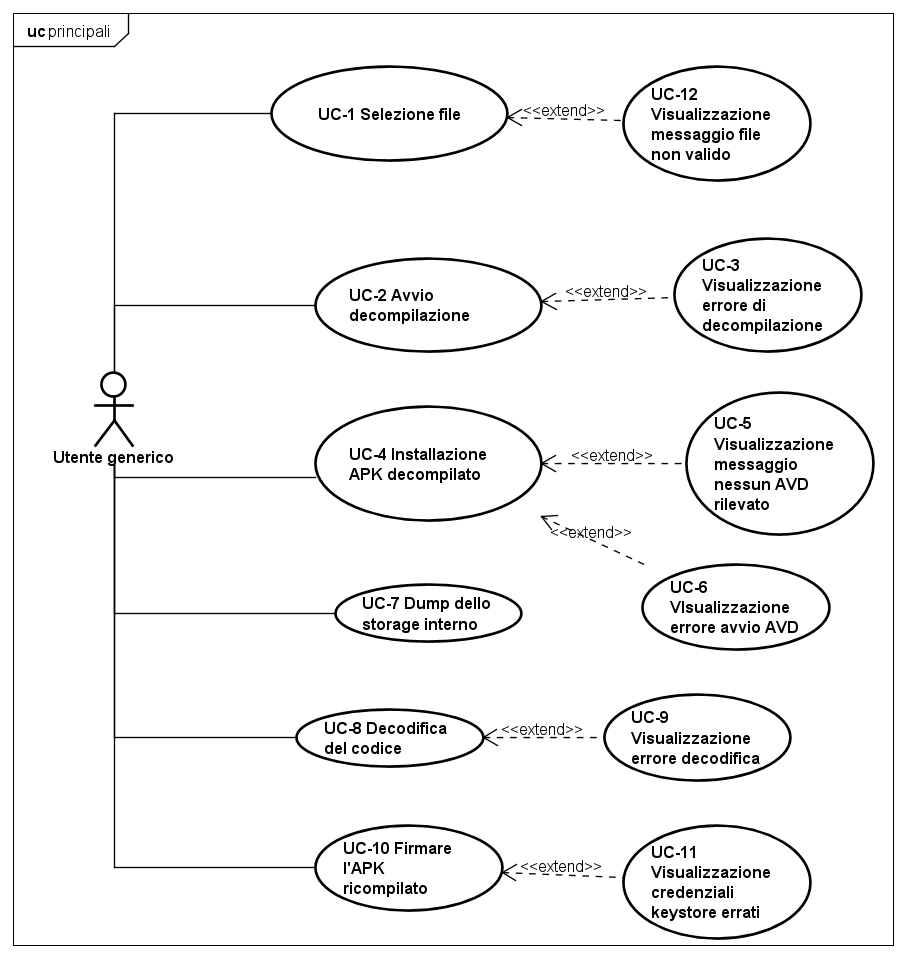
\includegraphics[width=10cm, height=8cm]{./immagini/usecase/uc_principali.png}
    \caption{Casi d'uso principali}
\end{figure}

\subsubsection{UC-10 Firmare l'APK ricompilato}\label{subsubsec:uc-10-firmare-l'apk-ricompilato}
\begin{itemize}
    \item \textbf{attori:} utente generico;
    \item \textbf{scopo:} permettere all'utente di firmare l'APK per la distribuzione;
    \item \textbf{descrizione:} dopo la ricompilazione si può firmare l'APK;
    \item \textbf{pre-condizioni:} la ricompilazione dell'APK è avvenuto correttamente;
    \item \textbf{post-condizioni:} l'APK è stata firmata correttamente;
    \item \textbf{flusso degli eventi principali:}
    \begin{itemize}
        \item UC-10.1 selezione keystore;
        \item UC-10.3 inserimento alias;
        \item UC-10.4 inserimento password.
    \end{itemize}
    \item \textbf{Estensione}
    \begin{itemize}
        \item UC-11 Visualizzazione credenziali keystore errati;
    \end{itemize}
\end{itemize}
\subsubsection{UC-10.1 Selezione keystore}\label{subsubsec:uc-10.1-selezione-keystore}
\begin{itemize}
    \item \textbf{attori:} utente generico;
    \item \textbf{scopo:} permettere all'utente di selezionare il keystore da utilizzare per firmare l'APK;
    \item \textbf{descrizione:} permettere all'utente di selezionare il keystore da utilizzare per firmare l'APK;
    \item \textbf{pre-condizioni:} la ricompilazione dell'APK è avvenuto correttamente;
    \item \textbf{post-condizioni:} è stato selezionato un file di tipo keystore corretto (estensione: \textbf{.jks});
    \item \textbf{flusso degli eventi principali:}
    \begin{itemize}
        \item l'utente seleziona la funzionalità per selezionare il keystore;
        \item l'utente seleziona il keystore;
    \end{itemize}
    \item \textbf{flussi secondari}
    \begin{itemize}
        \item UC-10.2 Visualizzazione messaggio file selezionato non valido;
    \end{itemize}
\end{itemize}
\subsubsection{UC-10.2 Visualizzazione messaggio file selezionato non valido}
\begin{itemize}
    \item \textbf{attori:} utente generico;
    \item \textbf{scopo:} mostrare all'utente il messaggio quando viene selezionato un file non valido;
    \item \textbf{descrizione:} l'utente, al quale è stato chiesto di selezionare un file di tipo keystore, potrebbe selezionare un file non valido;
    \item \textbf{pre-condizioni:} l'utente ha selezionato un file;
    \item \textbf{post-condizioni:} il messaggio di errore è stato mostrato;
    \item \textbf{flusso degli eventi principali:}
    \begin{itemize}
        \item l'utente visualizza il messaggio d'errore.
    \end{itemize}
\end{itemize}
\subsubsection{UC-10.3 Inserimento Alias}
\begin{itemize}
    \item \textbf{attori:} utente generico;
    \item \textbf{scopo:} permettere all'utente d'inserire l'alias della chiave da utilizzare;
    \item \textbf{descrizione:} l'utente deve inserire l'alias della chiave da utilizzare durante la firma dell'APK;
    \item \textbf{pre-condizioni:} l'utente ha selezionato un keystore valido;
    \item \textbf{post-condizioni:} l'utente ha inserito l'alias da utilizzare;
    \item \textbf{flusso degli eventi principali:}
    \begin{itemize}
        \item l'utente inserisce l'alias della chiave da utilizzare per firmare l'APK;
    \end{itemize}
\end{itemize}
\subsubsection{UC-10.4 Inserimento password}
\begin{itemize}
    \item \textbf{attori:} utente generico;
    \item \textbf{scopo:} permettere all'utente d'inserire la password del keystore;
    \item \textbf{descrizione:} l'utente deve inserire la password del keystore da utilizzare durante la firma dell'APK;
    \item \textbf{pre-condizioni:} l'utente ha selezionato un keystore valido;
    \item \textbf{post-condizioni:} l'utente ha inserito la password da utilizzare;
    \item \textbf{flusso degli eventi principali:}
    \begin{itemize}
        \item l'utente inserisce la password;
    \end{itemize}
\end{itemize}
\begin{figure}[H]
    \centering
    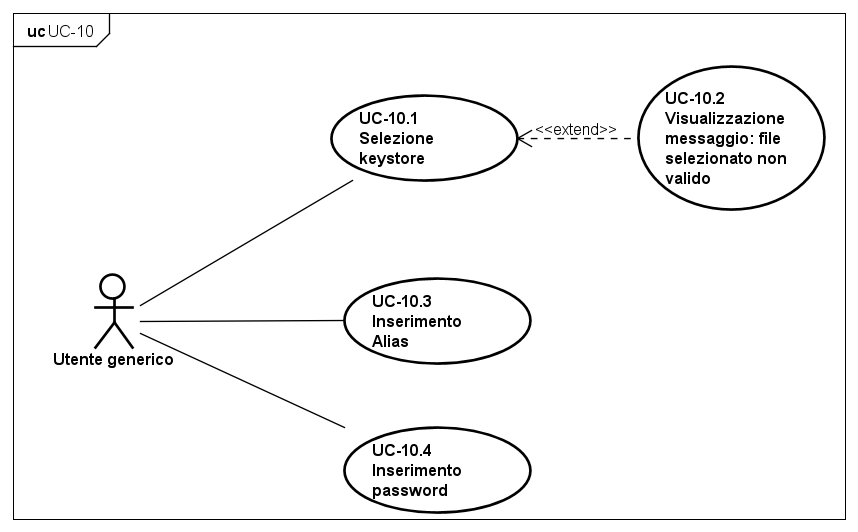
\includegraphics[width=10cm, height=8cm]{./immagini/usecase/uc_10.png}
    \caption{Sotto-casi d'uso UC-10 Firmare l'APK ricompilato}
\end{figure}

\subsubsection{UC-11 Visualizzazione credenziali keystore errati}\label{subsubsec:uc-11-visualizzazione-credenziali-keystore-errati}
\begin{itemize}
    \item \textbf{attori:} utente generico;
    \item \textbf{scopo:}  mostrare all'utente il messaggio di errore delle credenziali relativa al keystore;
    \item \textbf{descrizione:} per firmare l'APK l'utente è deve inserire dei credenziali, e quando quest'ultimi sono errati viene mostrato un messaggio di errore;
    \item \textbf{pre-condizioni:} l'utente ha selezionato la funzionalità per ricompilare l'APK;
    \item \textbf{post-condizioni:} l'utente ha visualizzato il messaggio di errore;
    \item \textbf{flusso degli eventi principali:}
    \begin{itemize}
        \item l'utente ha visualizzato l'errore;
    \end{itemize}
\end{itemize}

\subsubsection{UC-12 Visualizzazione messaggio file non valido}\label{subsubsec:uc-12-visualizzazione-messaggio-file-non-valido}
\begin{itemize}
    \item \textbf{attori:} utente generico;
    \item \textbf{scopo:} mostrare il messaggio di errore se seleziona un file non valido;
    \item \textbf{descrizione:} quando l'utente seleziona un file che non ha l'estensione APK un messaggio deve essere mostrato all'utente;
    \item \textbf{pre-condizioni:} l'utente ha selezionato un file non APK;
    \item \textbf{post-condizioni:} l'utente ha visualizzato il messaggio d'errore;
    \item \textbf{flusso degli eventi principali:}
    \begin{itemize}
        \item l'utente visualizza il messaggio d'errore.
    \end{itemize}
\end{itemize}
\subsubsection{UC-13 Decodifica dei file \textit{.dex} in file \textit{.java}}\label{subsubsec:uc-13-decodifica-dei-filetextitin-filetextit}
\begin{itemize}
    \item \textbf{attori:} utente generico;
    \item \textbf{scopo:} decodifica dei file .dex in class quindi da class in java;
    \item \textbf{descrizione:} dall'APK ricompilato si ottengono dei file \textit{.dex} che possono essere convertiti in \textit{.class} e quindi in \textit{.java};
    \item \textbf{pre-condizioni:} la decompilazione dell'APK \`{e} andata a buon fine;
    \item \textbf{post-condizioni:} la decodifica dei file \textit{.dex} in \textit{.java} \`{e} andata a buon fine;
    \item \textbf{flusso degli eventi principali:}
    \begin{itemize}
        \item l'utente seleziona la voce "Decodifica Dex".
    \end{itemize}
\end{itemize}
\begin{figure}[H]
    \centering
    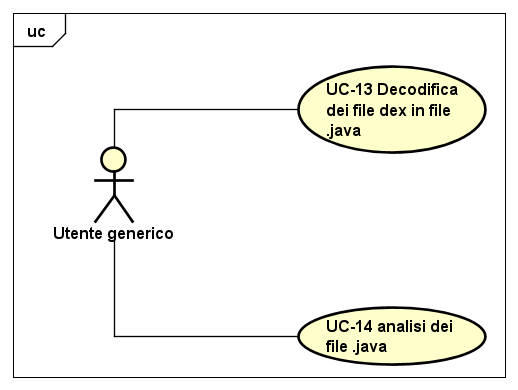
\includegraphics[width=10cm, height=8cm]{./immagini/usecase/UC-13_14.png}
    \caption{Casi d'uso 13 e 14}
\end{figure}
\subsubsection{UC-14 Analisi del codice \textit{.java}}\label{subsubsec:uc-14-analisi-del-codicetextit}
\begin{itemize}
    \item \textbf{attori:} attore generico;
    \item \textbf{scopo:} permettere di effettuare dell'analisi sul codice;
    \item \textbf{descrizione:} dopo aver ottenuto i file \textit{.java} eseguendo il caso d'uso UC-13, si potr\`{a} effettuare dell'analisi sul codice;
    \item \textbf{pre-condizioni:} la decodifica dei file \textit{.dex} in \textit{.java} \`{e} andata a buon fine;
    \item \textbf{post-condizioni:} viene generato un pdf con i risultati dell'analisi;
    \item \textbf{flusso degli eventi principali:}
    \begin{itemize}
        \item l'utente seleziona la voce "analyze";
        \item l'utente seleziona le opzioni di analisi;
        \item all'analisi completato, l'utente specifica dove posizionare il file pdf con i risultati dell'analisi;
        \item il file viene salvato nel percorso da lui specificato.
    \end{itemize}
\end{itemize}
\begin{figure}[H]
    \centering
    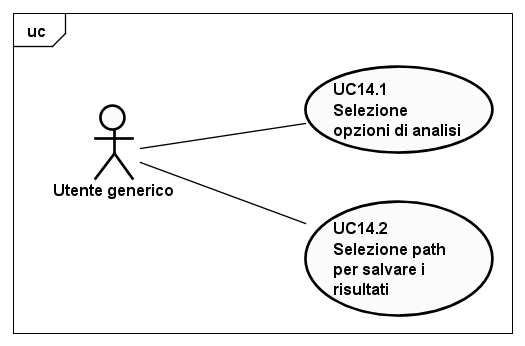
\includegraphics[width=10cm, height=8cm]{./immagini/usecase/uc_14_1_14_2.png}
    \caption{Sottocasi d'uso del caso d'uso 14}
\end{figure}


\section{Tracciamento dei requisiti}

\newcounter{rowcount}
\setcounter{rowcount}{0}
\newcounter{subCount}
\setcounter{subCount}{0}

\subsection{Classificazione}\label{subsec:classificazione}
Di seguito sono riportati i requisiti individuati durante l'attività di analisi.
Tali requisiti sono stati individuati dai casi d'uso e dai colloqui con il tutor interno \tutorAziendale.
I requisiti individuati sono stati divisi in:
\begin{itemize}
    \item \textbf{Requisiti funzionali:} insieme di requisiti che definiscono le azioni fondamentali che devono avvenire in grado di processare un input e di generare un output;
    \item \textbf{Requisiti dichiarativi:} insieme di requisiti che rappresentano un vincolo di natura realizzativa, normativa o contrattuale;
    \item \textbf{Requisiti qualitativi:} insieme di requisiti che garantiscono una certa qualità al prodotto e che indicano le best practice usate per la realizzazione.
\end{itemize}
Inoltre, a ogni requisito è stata assegnata un'importanza:
\begin{itemize}
    \item \textbf{Obbligatori:} requisito al quale non si può rinunciare, indispensabile per il corretto funzionamento del prodotto;
    \item \textbf{Desiderabile:} requisito non necessario ma che porta valore aggiunto al prodotto;
    \item \textbf{Facoltativo:} requisito che risulta essere relativamente utile oppure contrattabile con il proponente in un momento successivo.
\end{itemize}

\subsection{Requisiti funzionali}\label{subsec:requisiti-funzionali}
\renewcommand{\arraystretch}{1.5}
\begin{center}
    \begin{longtable}{ | c| C{7cm} |C{3cm} |}
        \hline
        \textbf{Identificativo} & \textbf{Descrizione} &\textbf{Fonte}\\\hline
        \idRequesiti{F-O} & Il tool deve permettere di selezionare un file APK.& UC-1\\\hline
        \idRequesitiSub{F-O} & Il tool deve permettere di mostrare un messaggio di errore se file selezionato non è valido. & UC-1\\\hline
        \setcounter{subCount}{0}

        \idRequesiti{F-O} & Il tool deve permettere di avviare la decompilazione dell'APK selezionato.& UC-2\\\hline
        \idRequesitiSub{F-O} & Il tool deve permettere di visualizzare un messaggio di decompilazione avvenuto con successo. & UC-2\\\hline
        \idRequesitiSub{F-O} & Il tool deve aggiungere il flag android:debuggable="true" nel AndroidManifest.xml del decompilato. & UC-2\\\hline
        \setcounter{subCount}{0}

        \idRequesiti{F-O} & Il tool deve permettere di visualizzare il messaggio di errore quando la decompilazione non è terminato con successo.& UC-3\\\hline
        \idRequesiti{F-O} & Il tool deve permettere d'installare l'APK decompilato e manomesso su un AVD. & UC-4 \\\hline
        \idRequesitiSub{F-D} & Il tool deve permettere di ricompilare l'APK decompilato.& UC-4\\\hline
        \idRequesitiSub{F-D} & Il tool deve permettere di avviare l'applicazione.& UC-4\\\hline
        \setcounter{subCount}{0}

        \idRequesiti{F-O} & Il tool deve permettere di selezionare un'AVD presente nel sistema.& UC-4.1 \\\hline
        \idRequesitiSub{F-O} & Il tool deve permettere di visualizzare l'elenco delle AVD presenti nel sistema operativo.& UC-4.1\\\hline
        \idRequesitiSub{F-O} & Il tool deve permettere di selezionare un'AVD presente nel sistema operativo.& UC-4.1\\\hline
        \idRequesitiSub{F-O} & Il tool deve permettere di confermare la selezione dell'AVD.& UC-4.1\\\hline
        \setcounter{subCount}{0}

        \idRequesiti{F-O} &Il tool deve permettere di visualizzare il messaggio quando non sono stati rilevati nessun AVD. & UC-5 \\\hline
        \idRequesiti{F-O} &Il tool deve permettere di visualizzare il messaggio di errore se l'AVD selezionato non si è avviato correttamente.& UC-6 \\\hline
        \idRequesiti{F-O} &Il tool deve permettere di fare il dump dello storage interna dell'applicazione.& UC-7 \\\hline
        \idRequesitiSub{F-O} & Il tool deve permettere di selezionare il path dove collocare i dati copiati.& UC-7\\\hline
        \setcounter{subCount}{0}

        \idRequesiti{F-D} &Il tool deve permettere di visualizzare i dex ottenuti dalla decompilazione.& UC-8\\\hline
        \idRequesitiSub{F-O} & Il tool deve permettere di visualizzare il messaggio quando la decodifica è avvenuto con successo.& UC-8\\\hline
        \idRequesitiSub{F-O} & Il tool deve permettere di far selezionare il dex che l'utente vuole decodificare.& UC-8.1\\\hline
        \idRequesitiSub{F-O} & Il tool deve permettere di confermare la selezione del dex da decodificare.& UC-8.1\\\hline
        \idRequesitiSub{F-O} & Il tool deve permettere di far selezionare il path di dove salvare i file ottenuti dalla decodifica.& UC-8.2\\\hline
        \setcounter{subCount}{0}

        \idRequesiti{F-O} &Il tool deve permettere di visualizzare il messaggio d'errore se la decodifica non è andato a buon fine.& UC-9 \\\hline

        \idRequesiti{F-F}& Il tool deve permettere di firmare l'APK ricompilato.& UC-10 \\\hline
        \idRequesitiSub{F-F} & Il tool deve permettere di selezionare un file di tipo keystore.&UC-10.1\\\hline
        \idRequesitiSub{F-F}& Il tool deve permettere di mostrare un messaggio di errore quando viene selezionato un file non keystore. & UC-10.2 \\\hline
        \idRequesitiSub{F-F} & Il tool deve permettere d'inserire l'alias della chiave da utilizzare.& UC-10.3 \\\hline
        \idRequesitiSub{F-F} & Il tool deve permettere d'inserire la password del keystore da utilizzare.& UC-10.4 \\\hline
        \setcounter{subCount}{0}

        \idRequesiti{F-F}& Il tool deve permettere di mostrare dei messaggi quando le credenziali inseriti non sono corretti.& UC-11 \\\hline
        \idRequesiti{F-O}& Il tool deve permettere di mostrare dei messaggi quando è stato selezionato un file non valido.& UC-12 \\\hline
        \idRequesiti{F-O}& Il tool deve permettere di decodificare i file \textit{.dex} in \textit{.java} & UC-13\\\hline
        \idRequesiti{F-O}& Il tool deve permettere di permettere di effettuare dell'analisi del codice java& UC-14 \\\hline
        \idRequesitiSub{F-O}& Il tool deve permettere di selezionare diverse opzioni di analisi &UC-14.1 \\\hline
        \idRequesitiSub{F-O}& Ilt tool deve permettere di selezionare il path dove collocare i risultati dell'analisi.& UC-14.2\\\hline
%        \idRequesiti{F-O}& Il tool deve permettere di & \\\hline

        \caption{Requisiti funzionali}
    \end{longtable}
\end{center}
\setcounter{rowcount}{0}

\subsection{Requisiti di vincolo}\label{subsec:requisiti-vincolo}
\renewcommand{\arraystretch}{1.5}
\begin{center}
    \begin{longtable}{ | c| C{7cm} |C{3cm} |}
        \hline
        \textbf{Identificativo} & \textbf{Descrizione} &\textbf{Fonte}\\\hline
        \idRequesiti{V-D} &Il tool può essere un tool da righe di commando & Colloquio col tutor aziendale.\\\hline
        \idRequesiti{V-D} &Il tool può essere un tool dotato di GUI & Colloquio col tutor aziendale.\\\hline
        \idRequesiti{V-D} &Il tool può essere sviluppato in JAVA & Colloquio col tutor aziendale.\\\hline
        \idRequesiti{V-F} &Il tool può essere sviluppato utilizzando i linguaggi funzionali.& Colloquio col tutor aziendale.\\\hline
        \caption{Requisiti di vincolo}
    \end{longtable}
\end{center}
\setcounter{rowcount}{0}

\subsection{Requisiti qualitativi}\label{subsec:requisiti-qualitativi}
\renewcommand{\arraystretch}{1.5}
\begin{center}
    \begin{longtable}{ | c| C{7cm} |C{3cm} |}
        \hline
        \textbf{Identificativo} & \textbf{Descrizione} &\textbf{Fonte}\\\hline
        \idRequesiti{Q-O}&Il codice sorgente deve essere versionato col sistema di versionamento dell'azienda ospitante. &Colloquio col tutor aziendale \\\hline
        \idRequesiti{Q-O}&Il code coverage dei test unitari deve superare 80\%.& Colloquio col tutor aziendale\\\hline
        \idRequesiti{Q-D}&Il code coverage dei test unitari deve essere 100\%.& Colloquio col tutor aziendale\\\hline
        \idRequesiti{Q-O}&Il Il codice sorgente deve essere sotto licenza GPL v3.& Colloquio col tutor aziendale\\\hline
        \caption{Requisiti qualitativi}
    \end{longtable}
\end{center}
\setcounter{subCount}{0}
\setcounter{rowcount}{0}
\subsection{Tracciamento fonte - requisiti}\label{subsec:tracciamento-fonte---requisiti}

\renewcommand{\arraystretch}{1.5}
\begin{center}
    \begin{longtable}{| C{6cm} |C{6cm}|} \hline
        \textbf{Fonte} & \textbf{Requisito} \\\hline
        UC-1 &
        \begin{itemize}
            \item R-1-F-O
            \item R-1.1-F-O
        \end{itemize}
        \\\hline
        UC-2 &
        \begin{itemize}
            \item R-2-F-O
            \item R-2.1-F-O
            \item R-2.2-F-O
        \end{itemize}
        \\\hline
        UC-3 &
        \begin{itemize}
            \item R-3-F-O
        \end{itemize}\\\hline
        UC-4 &
        \begin{itemize}
            \item R-4-F-O
            \item R-4.1-F-D
        \end{itemize}\\\hline
        UC-4.1 &
        \begin{itemize}
            \item R-5-F-O
            \item R-5.1-F-O
            \item R-5.2-F-O
            \item R-5.3-F-O
        \end{itemize}\\\hline
        UC-5 &
        \begin{itemize}
            \item R-6-F-O
        \end{itemize}\\\hline
        UC-6 &
        \begin{itemize}
            \item R-7-F-O
        \end{itemize}\\\hline
        UC-7 &
        \begin{itemize}
            \item R-8-F-O
            \item R-8.1-F-O
        \end{itemize}  \\\hline
        UC-8 &
        \begin{itemize}
            \item R-9-F-D
            \item R-9.1-F-O
        \end{itemize}\\\hline
        UC-8.1 &
        \begin{itemize}
            \item R-9.2-F-O
            \item R-9.3-F-O
        \end{itemize} \\\hline
        UC-8.2 &
        \begin{itemize}
            \item R-9.4-F-O
        \end{itemize}\\\hline
        UC-9 & \begin{itemize}
                   \item R-10-F-O
        \end{itemize}\\\hline
        UC-10 &
        \begin{itemize}
            \item R-10-F-O
        \end{itemize}
        \\\hline
        UC-11 &
        \begin{itemize}
            \item R-11-F-F
            \item R-11.1-F-F
            \item R-11.2-F-F
            \item R-11.3-F-F
            \item R-11.4-F-F
        \end{itemize}
        \\\hline


        UC-12 &
        \begin{itemize}
            \item R-12-F-F
        \end{itemize}
        \\\hline

        UC-1 &
        \begin{itemize}
            \item R-13-F-O
        \end{itemize}
        \\\hline

        UC-13 &
        \begin{itemize}
            \item R-14-F-O
        \end{itemize}\\\hline
        UC-14 &
        \begin{itemize}
            \item R-15-F-O
            \item R-15.1-F-O
            \item R-15.2-F-O
        \end{itemize}\\\hline
        Colloquio col tutor azienda &
        \begin{itemize}
            \item R-1-V-D,
            \item R-2-V-D,
            \item R-3-V-D,
            \item R-4-V-F,
            \item R-1-Q-O,
            \item R-2-Q-O,
            \item R-3-Q-D,
            \item R-4-Q-O
        \end{itemize} \\\hline
        \caption{Tracciamento fonte - requisiti}
    \end{longtable}
\end{center}

\subsection{Tracciamento requisito - fonte}\label{subsec:tracciamento-requisiti---fonte}
\renewcommand{\arraystretch}{1.5}
\begin{center}
    \begin{longtable}{| C{6cm} |C{6cm}|}
        \hline
        \textbf{Requisito} & \textbf{Fonte} \\\hline
        R-1-F-O&UC-1\\\hline
        R-1.1-F-O&UC-1\\\hline
        R-2-F-O&UC-2\\\hline
        R-2.1-F-O&UC-2\\\hline
        R-2.2-F-O&UC-2\\\hline
        R-3-F-O&UC-3\\\hline
        R-4-F-O&UC-4\\\hline
        R-4.1-F-D&UC-4\\\hline
        R-5-F-O&UC-4.1\\\hline
        R-5.1-F-O&UC-4.1\\\hline
        R-5.2-F-O&UC-4.1\\\hline
        R-5.3-F-O&UC-4.1\\\hline
        R-6-F-O&UC-5\\\hline
        R-7-F-O&UC-6\\\hline
        R-8-F-O&UC-7\\\hline
        R-8.1-F-O&UC-7\\\hline
        R-9-F-D&UC-8\\\hline
        R-9.1-F-O&UC-8\\\hline
        R-9.2-F-O&UC-8.1\\\hline
        R-9.3-F-O&UC-8.1\\\hline
        R-9.4-F-O&UC-8.2\\\hline
        R-10-F-O&UC-9\\\hline
        R-11-F-F&UC-10\\\hline
        R-11.1-F-F&UC-10.1\\\hline
        R-11.2-F-F&UC-10.2\\\hline
        R-11.3-F-F&UC-10.3\\\hline
        R-11.4-F-F&UC-10.4\\\hline
        R-12-F-F&UC-11\\\hline
        R-13-F-O&UC-12\\\hline
        R-14-F-O& UC-13\\\hline
        R-15-F-O & UC-14\\\hline
        R-15.1-F-O & UC-14\\\hline
        R-15.2-F-O & UC-14\\\hline
        R-1-V-D& Colloquio col tutor aziendale\\\hline
        R-2-V-D& Colloquio col tutor aziendale\\\hline
        R-3-V-D& Colloquio col tutor aziendale\\\hline
        R-4-V-F& Colloquio col tutor aziendale\\\hline
        R-1-Q-O& Colloquio col tutor aziendale\\\hline
        R-2-Q-O& Colloquio col tutor aziendale\\\hline
        R-3-Q-D& Colloquio col tutor aziendale\\\hline
        R-4-Q-O& Colloquio col tutor aziendale\\\hline
        \caption{Tracciamento requisiti - fonte}
    \end{longtable}
\end{center}